\documentclass[12pt, a4paper]{report}

\usepackage[czech]{babel}
\usepackage[utf8]{inputenc}
\usepackage[cp1250]{inputenc}
\usepackage[IL2]{fontenc}
\usepackage{graphicx}
\usepackage{float}


\title{\textbf{Automat řízení silniční křižovatky}}
\author{David Pivovar A13B0403P}

\begin{document}

%%%%%Titulni strana%%%%%%%%%%%%%%%%%%%%%%%%%%%%%%%%%%%%%%%%%%%%%%%%%%%%%%
\begin{titlepage}

\begin{figure}[t]
\centering
	
\includegraphics{image/logo_fav.jpg}
	\label{fig:logo_fav}
\end{figure}

\begin{center}
	{\large KIV/TI - Semestrální práce\\[0.3cm]}
	{\huge Automat řízení silniční křižovatky \\[1.7cm] }
\end{center}

\vfill

\begin{flushleft}
	{\large \textbf{David Pivovar}\\}
	{\large A13B0403P}
	\hfill
	{\large \today}
\end{flushleft}

\end{titlepage}
%%%%%%%%%%%%%%%%%%%%%%%%%%%%%%%%%%%%%%%%%%%%%%%%%%%%%%%%%%%


%%%%%Obsah%%%%%%%%%%%%%%%%%%%%%%%%%%%%%%%%%%%%%%%%%%%%%%%%%
\tableofcontents

\listoffigures
%%%%%%%%%%%%%%%%%%%%%%%%%%%%%%%%%%%%%%%%%%%%%%%%%%%%%%%%%%%


%%%%%Zadani%%%%%%%%%%%%%%%%%%%%%%%%%%%%%%%%%%%%%%%%%%%%%%%%
\chapter{Zadání}
Vytvořte automatový model řízení složité silniční křižovatky (alespoň šest semaforů pro auta, semafory pro chodce). Činnost automatu musí jít nějak ovlivnit (tlačítky pro chodce, detekcí čekajících aut, ...). Můžete udělat model reálné křižovatky, případně vymyslet vlastní. Jako vzor mohou sloužit např. křižovatky označené na mapě \url{https://www.google.com/maps/d/viewer\\?ll=49.746364,13.37182&t=h&ie=UTF8&msa=0&spn=0.018885,0.033431&z=15&hl=\\cs&mid=zD0-WWSE0ykI.kcdSYKD26j64}, nebo příklad vymyšlené křižovatky \url{http://home.zcu.cz/~jskala/ti/krizovatka.html}\\
\\
\noindent
Celé znění zadání práce je možné nalézt na následující url:\\
\url{http://home.zcu.cz/~jskala/ti/}

%%%%%%%%%%%%%%%%%%%%%%%%%%%%%%%%%%%%%%%%%%%%%%%%%%%%%%%%%%%


%%%%%Analyza ulohy%%%%%%%%%%%%%%%%%%%%%%%%%%%%%%%%%%%%%%%%%
\chapter{Analýza úlohy}

Rozhodl jsem se vytvořit automatový model křižovatky na Rokycanské mezi Plzeňským Prazdrojem a Hornbachem:

\begin{figure}[h]
	\centering
		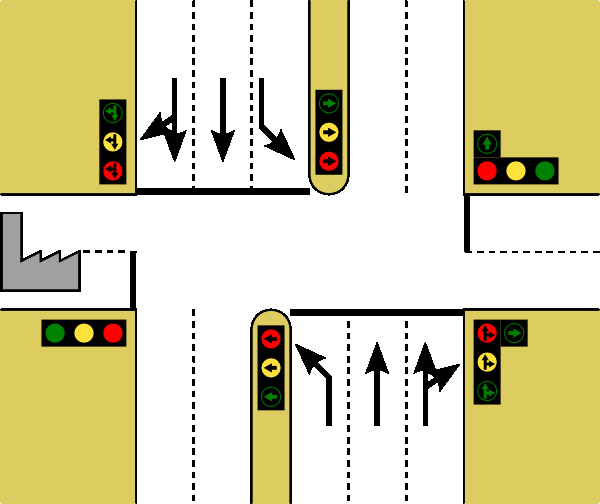
\includegraphics{image/krizovatka_Prazdroj_Hornbach.jpg}
	\caption{Křižovatka Rokycanská, mezi Pradrojem a Hornbachem}
	\label{fig:krizovatka_Prazdroj_Hornbach}
\end{figure}

\begin{itemize}
	\item na obrázku vlevo je vjezd do pivovaru
	\item při běžném provozu automat vůbec nedává zelenou pro jízdu z/do pivovaru
	\item zelená se zařadí jen na signál (detektor pod vozovkou, tlačítko ve vrátnici)
\end{itemize}

\noindent
Pro tuto křižovatku budou 3 stavy pro běžnou jízdu po Rokycanské a k Hornbachu:

\begin{figure}[!h]
	\centering
		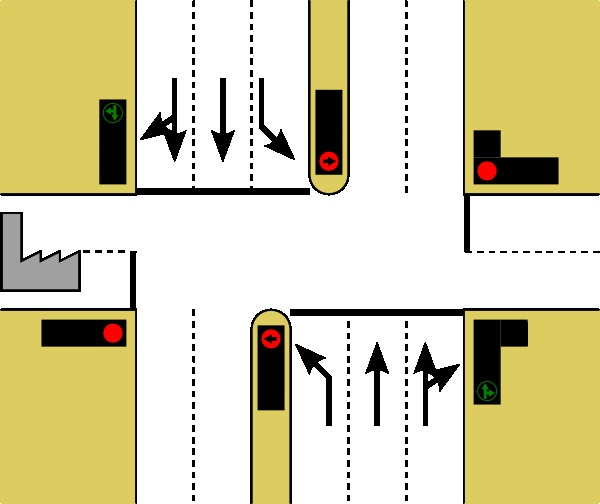
\includegraphics{image/S1_krizovatka.jpg}
	\caption{S1: přímý směr}
	\label{fig:S1_krizovatka}
\end{figure}

\begin{figure}[!h]
	\centering
		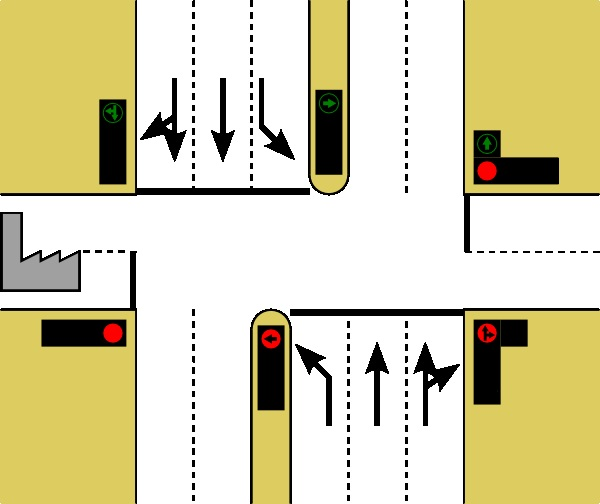
\includegraphics{image/S2_krizovatka.jpg}
	\caption{S2: Odbočení k Hornbachu}
	\label{fig:S2_krizovatka}
\end{figure}

\begin{figure}[!h]
	\centering
		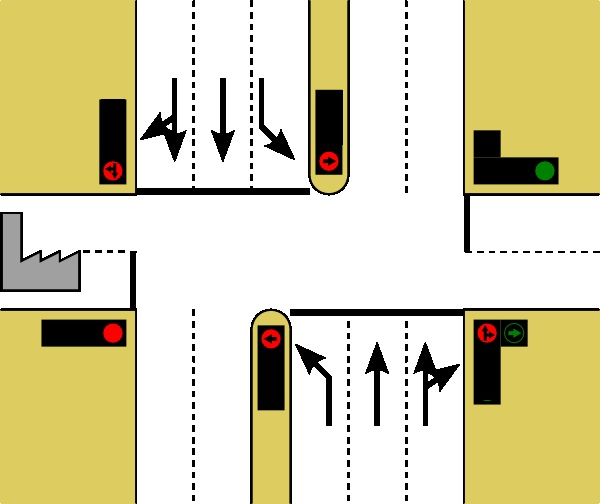
\includegraphics{image/S3_krizovatka.jpg}
	\caption{S3: Výjezd od Hornbachu}
	\label{fig:S3_krizovatka}
\end{figure}

\clearpage

\noindent
2 stavy pro jízdu z/do pivovaru, do kterých automat přejde po stisknutí ovládacího tlačítka na vrátnici pivovaru, nebo po aktivování senzoru na silnici:

\begin{figure}[!h]
	\centering
		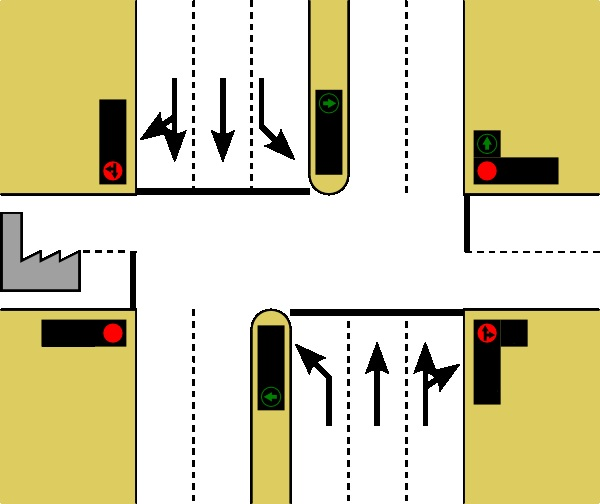
\includegraphics{image/S4_krizovatka.jpg}
	\caption{S4: Vjezd do pivovaru}
	\label{fig:S4_krizovatka}
\end{figure}

\begin{figure}[!h]
	\centering
		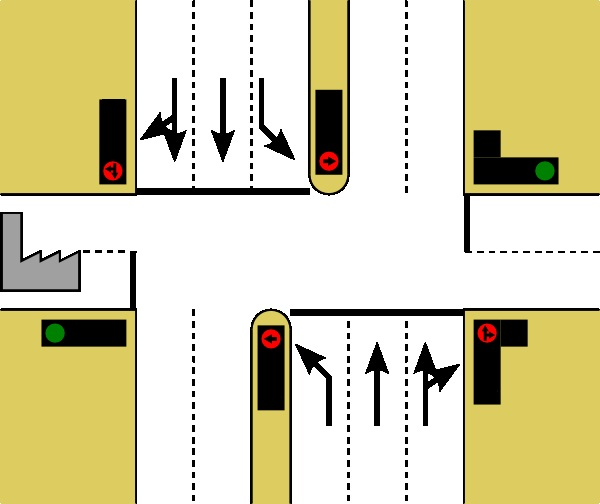
\includegraphics{image/S5_krizovatka.jpg}
	\caption{S5: Výjezd z pivovaru}
	\label{fig:S5_krizovatka}
\end{figure}

\clearpage

\noindent
Ke každému stavu existuje ekvivalent s oranžovým světlem namísto zeleného.\\

\begin{figure}[!h]
	\centering
		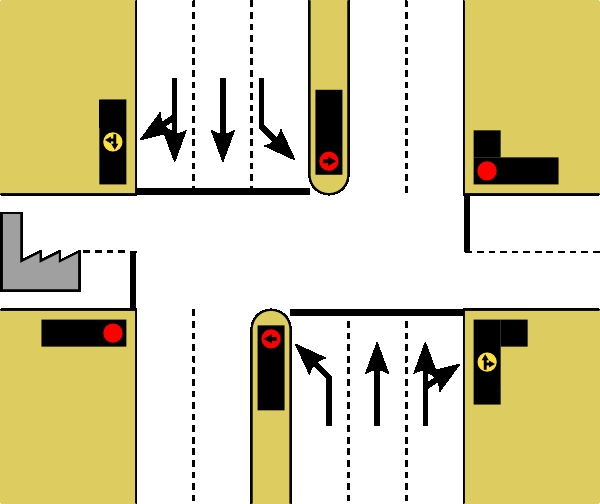
\includegraphics{image/S1+_krizovatka.jpg}
	\caption{S1': oranžová pro přímý směr}
	\label{fig:S1+_krizovatka}
\end{figure}

\noindent
Nejdéle setrvá automat ve stavu S1 pro jízdu v přímém směru, čas {\b Td}. Stav S2 pro odbočení k Hornbachu a stav S3 pro vyjetí od Hornbachu čas {\b Th}, stav S4 a S5 pro jízdu z/do pivovaru čas {\b Tp}. Nejkratší dobu pak setrvá ve stavech pro oranžové světlo, čas {\b To}\\
{\b Td >> Th >> Tp >> To}\\
\\
Tlačítka pro obsluhu jízdy z/do pivovaru jsou pojmenovány {\b b4, b8}, senzory {\b s4, s8}, podle semaforu, kterému jsou určeny.

%%%%%%%%%%%%%%%%%%%%%%%%%%%%%%%%%%%%%%%%%%%%%%%%%%%%%%%%%%%


%%%%%Automatový model%%%%%%%%%%%%%%%%%%%%%%%%%%%%%%%%%%%%%%
\chapter{Automatový model}

\section{Přechodový graf}

\begin{figure}[!h]
	\centering
		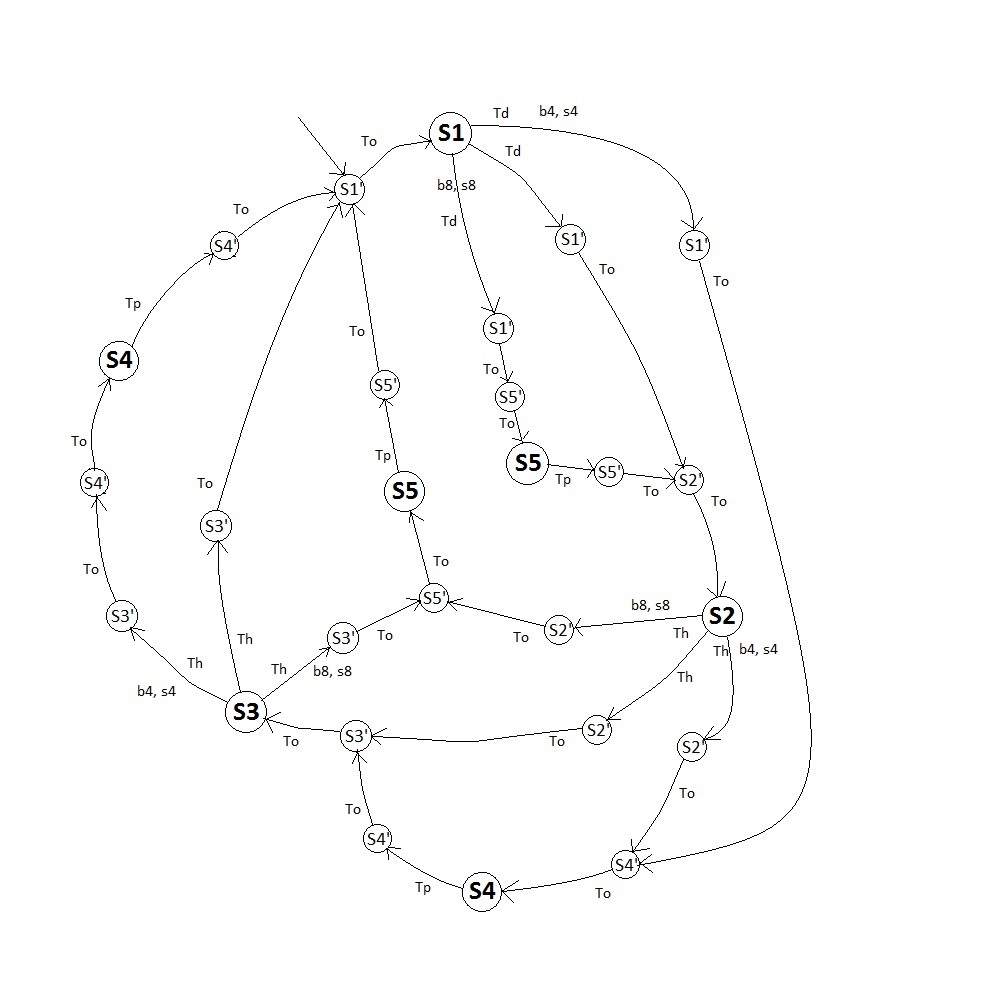
\includegraphics[width=0.80\textwidth]{image/prechodovy_graf.jpg}
	\caption{Přechodový graf}
	\label{fig:prechodovy_graf}
\end{figure}


\clearpage

\section{Tabulka stavů}

\begin{table}[!h]
	\centering
		\begin{tabular}{1||1|1|1|1|1|1|1|1}
		
		Stav & 1 & 2 & 3 & 4 & 5 & 6 & 7 & 8\\
		\hline \hline
		S1 & 1 & -1 & 1 & -1 & -1 & -1 & -1 & -1\\
		\hline
		S1' & 0 & -1 & 0 & -1 & -1 & -1 & -1 & -1\\
		\hline
		S2 & 1 & 1 & -1 & -1 & -1 & -1 & 1 & -1\\
		\hline
		S2' & 0 & 0 & -1 & -1 & -1 & -1 & -1 & -1\\
		\hline
		S3 & -1 & -1 & -1 & -1 & 1 & 1 & -1 & -1\\
		\hline
		S3' & -1 & -1 & -1 & -1 & -1 & 0 & -1 & -1\\
		\hline
		S4 & -1 & 1 & -1 & 1 & -1 & -1 & 1 & -1\\
		\hline
		S4' & -1 & 0 & -1 & 0 & -1 & -1 & -1 & -1\\
		\hline
		S5 & -1 & -1 & -1 & -1 & -1 & 1 & -1 & 1\\
		\hline
		S5' & -1 & -1 & -1 & -1 & -1 & 0 & -1 & 0\\
		
		
		\end{tabular}
\end{table}

\begin{itemize}
	\item 1...zelená
	\item 0...oranžová
	\item -1...červená/zhasnuto
\end{itemize}

\begin{figure}[!h]
	\centering
		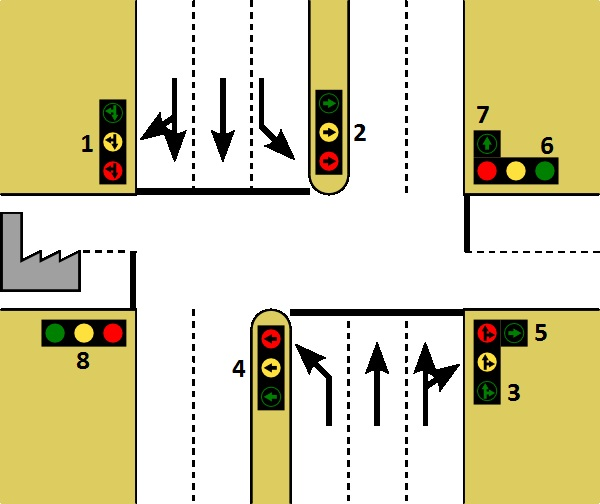
\includegraphics{image/oznaceni_semaforu.jpg}
	\caption{Označení semaforů}
	\label{fig:oznaceni_semaforu}
\end{figure}

%%%%%%%%%%%%%%%%%%%%%%%%%%%%%%%%%%%%%%%%%%%%%%%%%%%%%%%%%%%


%%%%%Implementace%%%%%%%%%%%%%%%%%%%%%%%%%%%%%%%%%%%%%%%%%%
\chapter{Implementace}
Pro každý nečárkovaný stav jsem vytvořil jednu metodu, kdy jsem nečárkovaný stav obalil čárkovaným, přidal časovač a podmínku, který stav bude následovat\\
\\
Struktura metody pro S1:

\begin{itemize}
\item S1'
\item	časovač To
\item S1
\item časovač Td
\item S1'
\item časovač To
\item podmínka pro následující stav
\end{itemize}
\\
\noindent
Časovač je řešen porovnáním systémového času. Zvolená perioda se násobí koeficientem pro daný čas.\\
Koeficienty časů:

\begin{itemize}
\item Td = 8
\item	Th = 6
\item Tp = 4
\item To = 1
\end{itemize}

\noindent
Podmínka u stavů běžného provozu vyhodnocuje, jestli nebylo zmáčknuto tlačítko pro jízdu z/do pivovaru. Podmínka u stavů pro jízdu z/do pivovaru vyhodnocuje do jakého stavu má pokračovat.\\
Tlačítka nastavují pomocné proměnné, které jsou vyhodnocovány v  podmínkách.


%%%%%%%%%%%%%%%%%%%%%%%%%%%%%%%%%%%%%%%%%%%%%%%%%%%%%%%%%%%

%%%%%Uzivatelska priruca%%%%%%%%%%%%%%%%%%%%%%%%%%%%%%%%%%%
\chapter{Uživatelská příručka}

Program je psán v jazyce C# v prostředí Microsof Visual Studio 2013 Ultimate.

\section{Překlad a spuštění programu}
Překlad lze provést v Microsoft Visual Studio Expres 2013 for Windows, Microsoft Visual Studio Professional/Premium/Ultimate 2013. Překlad ve starších verzích Microsoft Visual Studia jsem nezkoušel, ale pravděpodobně by měl fungovat.\\
\\
Program se spustí \uv{Krizovatka.exe}.

\section{Ovládání programu}
Po spuštění programu se automat uvede do chodu tlačítkem \uv{Go}, kdy začíná stavem S1'.\\
Tlačítko \uv{b4, s4} slouží jako tlačítko na vrátnici pivovaru či jako senzor ve vozovce pro vjezd do pivovaru, tlačítko \uv{b8, s8} pro výjezd z pivovaru.\\
Tlačítkem \uv{Close} se program ukončí.\\
\\
Pomocí číselné hodnoty lze nastavit velikost periody časů rozsvícení semaforů.


%%%%%%%%%%%%%%%%%%%%%%%%%%%%%%%%%%%%%%%%%%%%%%%%%%%%%%%%%%%


%%%%%Zaver%%%%%%%%%%%%%%%%%%%%%%%%%%%%%%%%%%%%%%%%%%%%%%%%%
\chapter{Závěr}

Model automatu i program splňují zadání.\\
Model automatu lze vylepšit přidáním senzorů aut, které by upravovaly časovače podle počtu aut pro daný směr. Dále by bylo vhodné odstranit zhasínání a rozsvěcení zelené semaforu mezi dvěma stavy, pokud má v obou stavech svítit zelená.\\
GUI programu by se dalo vylepšit zobrazením jízdních pruhů či rozložením semaforu do tří barevných oken místo aktuálního jednoho.
%%%%%%%%%%%%%%%%%%%%%%%%%%%%%%%%%%%%%%%%%%%%%%%%%%%%%%%%%%%


\end{document}
